% v2-acmtog-sample.tex, dated March 7 2012
% This is a sample file for ACM Transactions on Graphics
%
% Compilation using 'acmtog.cls' - version 1.2 (March 2012), Aptara Inc.
% (c) 2010 Association for Computing Machinery (ACM)
%
% Questions/Suggestions/Feedback should be addressed to => "acmtexsupport@aptaracorp.com".
% Users can also go through the FAQs available on the journal's submission webpage.
%
% Steps to compile: latex, bibtex, latex latex
%
% For tracking purposes => this is v1.2 - March 2012
\documentclass{acmtog} % V1.2

%\acmVolume{VV}
%\acmNumber{N}
%\acmYear{YYYY}
%\acmMonth{Month}
%\acmArticleNum{XXX}
%\acmdoi{10.1145/XXXXXXX.YYYYYYY}




%\markboth{Ranking the importance of node in a complex network}

\title{Ranking the importance of node in a complex network} % title

\author{Feng Chang {\upshape and} Guoyi Qu
\affil{Shanghai Jiao Tong University}
% NOTE! Affiliations placed here should be for the institution where the
%       BULK of the research was done. If the author has gone to a new
%       institution, before publication, the (above) affiliation should NOT be changed.
%       The authors 'current' address may be given in the "Author's addresses:" block (below).
%       So for example, Mr. Fogarty, the bulk of the research was done at UIUC, and he is
%       currently affiliated with NASA.
}
\begin{document}

\maketitle
\section{Introduction}
Complex networks provide convenient models for complex systems in biology, physics, and social sciences.\cite{ref1} Many mechanisms of complex networks such as spreading dynamics, cascading reactions, and network synchronization are highly affected by a tiny fraction of so-called important nodes. Identifying the most important nodes or ranking the node importance by using the method of quantitative analysis in large scale networks is thus very significant.

In this article, we introduce a ranking method using PageRank and Learning-To-Rank for complex networks. Different from other ranking methods defined in text or database systems, links or the structure information of the network are significantly explored. For most of the ranking methods in networks, ranking scores are defined in a way that can be propagated in the network. Therefore, the rank score of an object is determined by other objects in the network, usually with stronger influence from closer objects and weaker influence from more remote ones.\cite{ref2}

\section{Background}
PageRank, one of the most popular ranking algorithms, has been originally devised to rank web sites in search engine results4. The algorithm acts on unipartite directed networks and builds on the circular idea “A node is important if it is pointed by other important nodes”. 

Larry Page and Sergey Brin developed PageRank at Stanford University in 1996 as part of a research project about a new kind of search engine. The name "PageRank" plays off of the name of developer Larry Page, as well as of the concept of a web page.\cite{ref3}

The mathematics of PageRank are entirely general and apply to any graph or network in any domain. Thus, PageRank is now regularly used in bibliometrics, social and information network analysis, and for link prediction and recommendation. It's even used for systems analysis of road networks, as well as biology, chemistry, neuroscience, and physics.

\section{Motivation}
The widespread usage of PageRank motivates us to ask: whether the PageRank is a perfect algorithm for ranking? The result is obviouly no. At the time we tried to implement the PageRank algorithm in the beginning of project, plenty of problems arose. In order to optimize the PageRank, we tried to combine PageRank with Machine Learning methods.

\section{Related Work}
Methods for ranking in networks can be categorized according to several aspects, such as global ranking vs. query-dependent ranking, based on whether the ranking result is dependent on a query; ranking in homogeneous information networks vs. ranking in heterogeneous information networks, based on the type of the underlying networks; importance-based ranking vs. proximity-based ranking, based on whether the semantic meaning of the ranking is importance related or similarity/promximity related; and unsupervised vs. supervised or semi-supervised, based on whether training is needed.

Our project focused on the webpage ranking. In the early time of Internet, search engines treat Internet web pages as text, mainly using traditional information retrieval sorting models, such as BM25\cite{ref4}
, LMIR(Language Model for IR)\cite{ref5}, etc. Later, search engines began to use the ultra-text structure of the Internet to calculate the importance of web pages. The representative algorithms are PageRank and so on. With the continuous development of search technology, more and more factors need to be considered in page sorting. It is not realistic to expect to manually integrate hundreds of factors into sorting formulas. Researchers have begun to try to use supervised machine learning methods to sort The factors are integrated, that is, the machine learning method is used to train the sorting model from the user's annotation or search log data, which is called sorting learning. However, in the past, the sorting learning research solved the problems of automatic learning and the integration of a large number of sorting features. However, in general, the relevance and importance of the content are ranked, and the interaction between documents is neglected.

\section{Problem Formulation}
Given a grapg G=(V,E), a set of nodes T(G) where each node has features $f_1,f_2,\cdots, f_k$, we try to fina relative importance of nodes in a graph with respect to a set of root nodes R and a certain queries. The output is permutation on features vectors $\pi=sort({f(x_i)}_{i=1}^n)$

We aim to train a (local) ranking model f(q,v)=f(x) that can assign a score to a given query node pair q and v, or equivalently to a given feature vector x. The architecture of this project is as follows:
\begin{figure}[htbp]
    \centering
    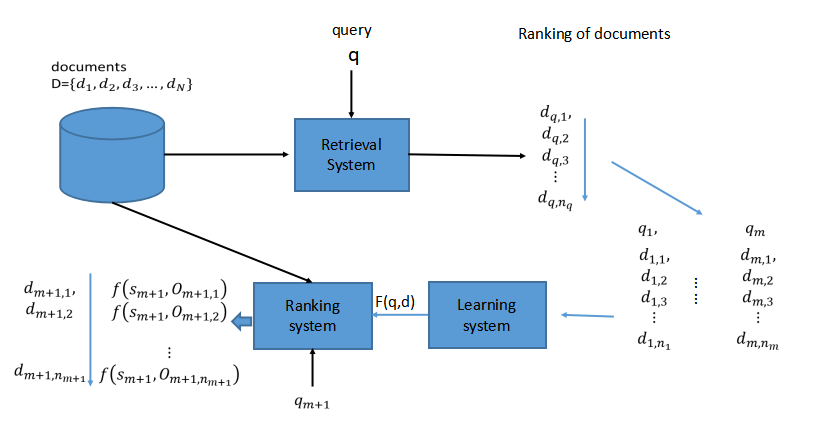
\includegraphics[width = 3in]{1.png}
    \caption{project architecture}
    \label{fig:my_label}
\end{figure}
We use MAP(Mean average precision) \cite{ref6} to evaluate the effort of ranking model. Mean average precision for a set of queries is the mean of the average precision scores for each query. The formula of MAP is as follows:
\begin{eqnarray}
  MAP=\frac{\sum_{q=1}{Q}AveP(q)}{Q}
  \label{eq:MAP_formula}
\end{eqnarray}  
where Q is the number of queries.

\section{PageRank algorithm}
PageRank (PR) is an algorithm used by Google Search to rank web pages in their search engine results. PageRank was named after Larry Page,one of the founders of Google. PageRank is a way of measuring the importance of website pages.
\subsection{Basic Idea of PageRank}
If the web page T has a connection to web page A, it indicates that the owner of T considers A to be more important, thereby assigning a part of the importance score of T to A. This importance score is:
\begin{eqnarray}
  PrScore(T)= \frac{PR(T)}{L(T)}
  \label{eq:importance_Score}
\end{eqnarray}    
Where PR(T) is the PageRank value of T and L(T) is the number of chained T.

Then the PageRank value of A is the accumulation of a series of page importance score values similar to T.

That is, the number of votes for a page is determined by the importance of all the links to its pages. A hyperlink to a page is equivalent to voting for the page. The PageRank of a page is obtained by a recursive algorithm of the importance of all the links to its pages (linked into the page). A page with more links will have a higher level. On the contrary, if a page does not have any links to the page, then it has no level.

For an Internet page A, the calculation of PageRank of the page is based on the following two basic assumptions:  Quantity hypothesis: In the Web graph model, if the number of other web pages received by a page node points to more, then this The more important the page is.  Quality Assumption: The quality of the links to page A is different, and the pages with high quality will pass more weights to other pages through links. So the higher the quality of the page points to page A, the more important page A is.
\subsection{PageRank Algorithm}
The algorithm of PageRank is defined as follows:
\begin{enumerate}
    \item [(1)]Define a vector v of initial rank value for each node. Because the user initially accesses the node randomly, the initial value of each node is equal. For example, the are N nodes, the rank value of each node is set to 1/N.
    \item [(2)]A transfer matrix M is generated based on the links between the nodes. When the user accesses node, he randomly accesses the next node through a link on the node. The value of this matrix M[i][j] represents the probability from node i to node j.
    \item [(3)] Use v=Mv instead of the vector of the rank value. This gives the probability distribution of the first transfer access to each node.
    \item [(4)] Repeat step (3). The vector of rank value will eventually converge, which is provable. This converged vector is the rank value we want.
\end{enumerate}
\subsection{PageRank Implementation}
The PageRank algorithm is not complex, its complete formula is as follows:
\begin{eqnarray}
  PageRank(p_i)=\frac{1-q}{N}+q\sum_{p_j}\frac{PageRank(p_j)}{L(p_j)}
  \label{eq:PageRank_formula}
\end{eqnarray}  
where $p_1,p_2,\cdots,p_N$ represent the researched page, $M(p_i)$ is the amount of pages connected to $p_i$, $L(p_j)$ is the amount of pages connected to $p_j$ and N is the amount of all pages.
\subsection{Problem of PageRank}
The implementation of PageRank is not complex, however, we noticed some serious problems of PageRank that leads to low availability of PageRank.
\begin{enumerate}
    \item [(1)]Dead end: in most cases, the web is not a strongly connected graph. Many nodes are not linked to other nodes. This will cause the resulting vector to be zeroed.
    \item [(2)] Spider trap: there are some trap nodes on the web that only link to themselves. Such nodes will continuously absorb the rank values of other nodes until the become zero.
    \item [(3)] Too many nodes: there are tens of millions of nodes in the web. This can result in slow calculation and insufficient memory.
    \item [(4)] There is no distinction between in-site navigation links. Many nodes have a lot of links to other nodes in the site, called in-site navigation links. Compared with the links between different sites, these links are definitely the latter to better reflect the transfer relationship of rank values.
    \item [(5)]There are no filtered ad links and feature links (such as the usual "Share to Weibo"). These links usually have no real value, the former links to the ad page, which often links to the home page of a social site.
    \item [(6)]It is not friendly to new nodes. A new node has a relatively small general chain, and even if its content is of high quality, it takes a long time to become a high PR node.
\end{enumerate}
\subsection{Improvement of PageRank}
Due to the problem we described above,we tried to reduce the disadvantages caused by the problem in two ways.
\subsubsection{Storage mode change}
 Because a node often has only a few dozen links, we use adjacency list instead of matrix.
 \subsubsection{Make it more realistic}
 When we go online, we don't just jump to the next page based on the link provided by the current page, we also enter a link at the top of the browser to jump. The same as this, we let it has a certain probability of not browsing the current node content and randomly jumping to other nodes. That is, in the algorithm, v=Mv becomes v=pMv+(1-p)(1/N). p indicates the probability of the link to jump after entering a node. N is the number of nodes. This will not fall into dead ends and spider trap.

\section{ListNet}
For the traditional sorting model, if the parameters are more, it will make the empirical method adjustment particularly difficult. So using machine learning to solve this problem may make the problem easier. There are three common ways to solve the sorting problem with machine learning:
    
\begin{enumerate}
    \item [1] Pointwise
    \item [2] Pairwise
    \item [3] Listwise
\end{enumerate}
They are different in their loss function where pointwise focuses on a single document at a time, pairwise looks at a pair of documents at a time and listwise looks at the entire list of documents. However, due to different loss functions, both pairwise and pointwise ranking methods don't take the order relationship between documents, we use listwise in this project.
\subsection{Listwise approach}
Suppose we have m querys:
\begin{eqnarray}
  Q=(q^{(1)}, q^{(2)},q^{(3)},\cdots,q^{(m)})
\end{eqnarray}
each query has n documents associated with it(different query has different n).
\begin{eqnarray}
  d^{(i)}=(d_1^{(i)},d_2^{(i)},\cdots,d_n^{(i)})
\end{eqnarray}
From each document in query, we can get the true relevance score of each document and query according to the specific application scenario.
\begin{eqnarray}
  y^{(i)}=(y_1^{(i)},y_2^{(i)},\cdots,y_n^{(i)})
\end{eqnarray}
We can get the feature vector of this document from document pair $(q^{i},d_j^{i})$, then we can get all feature vectors of this query:
\begin{eqnarray}
 x^{(i)}=(x_1^{(i)},x_2^{(i)},\cdots,x_n^{(i)})
\end{eqnarray}
And we can know the true relevance score of each document:
\begin{eqnarray}
  y^{(i)}=(y_1^{(i)},y_2^{(i)},\cdots,y_n^{(i)})
\end{eqnarray}
From this we can build training samples:
\begin{eqnarray}
  T=\{(x^{(i)},y^{(i)}) \}_{i=1}{m}
\end{eqnarray}
Then, we can notice that the training samples is $(x^{(i)},y^{(i)})$, which is the difference between pairwise, pointwise and listwise.
Then, our goal is to minimize the true score and predicted score error. That is 
\begin{eqnarray}
  \sum_{i=1}{m}L(y^{(i)},z^{(i)})
\end{eqnarray}
where L is the loss function of listwise.

\subsection{Probability Model}
In general, we take a kind of rank possibility as 
\begin{eqnarray}
  P_s(\pi)= \prod_{j=1}^{n} \frac{\phi(S_{\pi}(j))}{\sum_{k=j}^n \phi(S_{\pi}(k))}
\end{eqnarray}
where $\phi()$ is a function of increment and constant greater than 0, $S_n(j)$ is the score of the documents ranking j. It is easy to understand, however, when it comes to large amount of documents, its computational complexity is O(n!), hard to calculate. So we tried to use top-K Probability Model, which means we only need to calculate the k documents ranking the front k in all documents. The computational complexity of top-k Probability Model is $N!/(N-K)!$, much lower than the N! of the former model. The formula of top-k is as follows:
\begin{eqnarray}
  P_s(\pi)=\prod_{j=1}{K}\frac{\phi(S_{]pi}(j))}{\sum_{k=j}^{n}\phi(S_{\pi}(k))}
\end{eqnarray}
For N!/(N−k)! N!/(Nk)!N!/(N−k)! There are different arrangements, N!/(N−k)! N!/(Nk)! N!/(N−k)! Arranges the prediction probability to form a probability distribution, and then calculates the corresponding permutation probability from the true correlation score to obtain the true permutation probability distribution. From this we can use cross−entropy cross-entropycross−entropy to calculate the distance between the two distributions as a loss function:
\begin{eqnarray}
  L(y^{(i)},z^{(i)})=-\sum_{j=1}^nP_{y^{(i)}}(j)\log(P_z^{(i)}(j)))
\end{eqnarray}
In this project, we just take the function $\phi$ as $exp$ function, and K=1, then the arrangement probability will change to 
\begin{eqnarray}
  P_s(\pi)=\frac{exp(s_{\pi}(j)}{\sum_{k=j}{n} exp(S_{\pi}(k))}
\end{eqnarray}
Like softmax Function.

\subsection{Neural Network}
We use Neural Network as a model and Gradient Descendant as optimization in this project. Neural Network is good at dealing with constructing a model of nonlinear complex relationships and inferring an unknown relationship from unknown data, which is suitable for this ranking job, so we choose it as the model. The architecture of the model is as follows:

\begin{figure}[htbp]
    \centering
    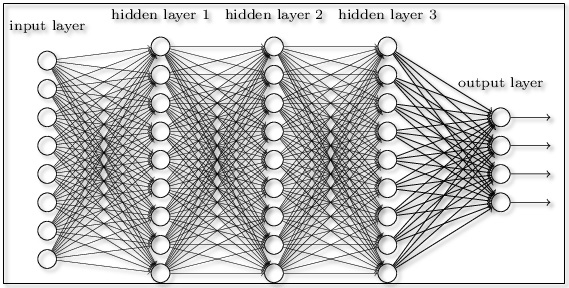
\includegraphics[width = 3in]{2.png}
    \caption{Neural Network Architecture}
\end{figure}

We use 3 fully connected layer with relu activation function. And dropout some neurons after each layer to accelerate and prevent overfitting.

\section{Experiment}
\subsection{Dataset}
We use LETOR4.0 dataset for our project. LETOR is a package of benchmark data sets for research on Learning TO Rank, which contains standard features, relevance judgments, data partitioning, evaluation tools, and several baselines. It uses the Gov2 web page collection (~25M pages) and two query sets from Million Query track of TREC 2007 and TREC 2008. We call the two query sets MQ2007 and MQ2008 for short. There are about 1700 queries in MQ2007 with labeled documents and about 800 queries in MQ2008 with labeled documents.\cite{ref7}

Link graph (~ 480M) of Gov2 collection. Each line contains the inlinks of a web page. We use it to calculate the PageRank values.

MQ2008-list(~ 80M) contains some queries and documents relations, we use it to evaluate our Ranking model.An example is shown as follow.

==============================

-1 qid:18219 1:0.022594 2:0.000000 3:0.250000 4:0.166667 … 45:0.004237 46:0.081600 #docid = GX004-66-12099765 inc = -1 prob = 0.223732

0 qid:18219 1:0.027615 2:0.500000 3:0.750000 4:0.333333 … 45:0.010291 46:0.046400 #docid = GX004-93-7097963 inc = 0.0428115405134536 prob = 0.860366

-1 qid:18219 1:0.018410 2:0.000000 3:0.250000 4:0.166667 … 45:0.003632 46:0.033600 #docid = GX005-04-11520874 inc = -1 prob = 0.0980801

==============================

\subsection{Complex network PageRank value}
We use linked list to implement this part. The algorithm we have introduced in detail. The input is Link graph (~ 480M) of Gov2 collection, and the output is each node id with its PageRank value.

\begin{figure}[htbp]
    \centering
    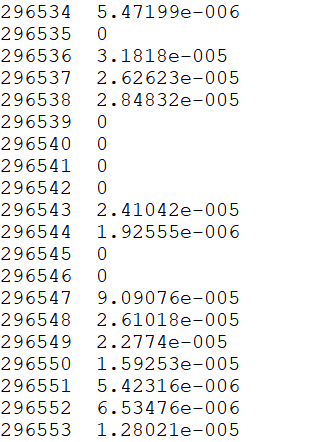
\includegraphics[width = 2in]{3.png}
    \caption{PageRank Result}
\end{figure}

The only question is that the number of nodes is so many (approximately 25,000,000) that it takes us lots of time to get PageRank value list.

\subsection{Listnet without PageRank value}
We divide all queries into five parts, three of which are training set, one part is test set and the other part is vali set. In this part, we only used some features of documents, such as TF(Term frequency) of body,TF of anchor, IDF(Inverse document frequency) of body,DL(Document length) of URL and did't add the representing the relationship weight between documents. And in this way, we get the loss and accuracy as follows:

\begin{figure}[htbp]
    \centering
    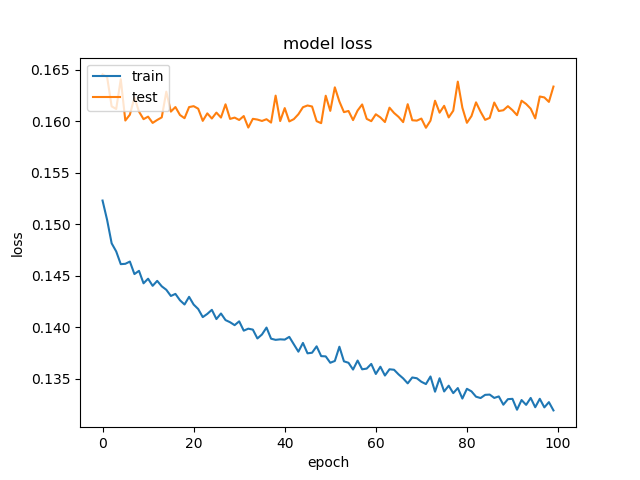
\includegraphics[width = 1.8in]{8.png}
    \caption{Model loss no pagerank}
\end{figure}

\begin{figure}[htbp]
    \centering
    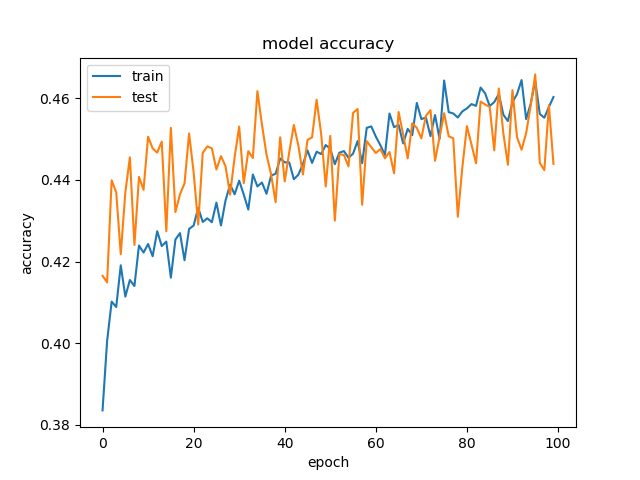
\includegraphics[width = 1.8in]{9.png}
    \caption{Model accuracy no pagerank}
\end{figure}
We choose the model with the least loss, the minimum loss is 0.142263 , and the accuracy with this model is 0.386446.

\subsection{Listnet with PageRank value}
In this part, we tried to add the features associated with the relationship weight between different webpages, such as PageRank value, Inlink number, Outlink number, Number of child page. Then use listnet to get a model and evaluate its accuracy.
\begin{figure}[htbp]
    \centering
    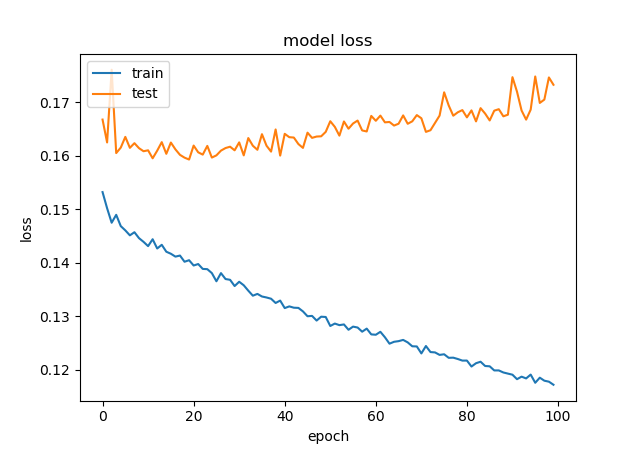
\includegraphics[width = 1.8in]{10.png}
    \caption{Model loss with pagerank}
\end{figure}

\begin{figure}[htbp]
    \centering
    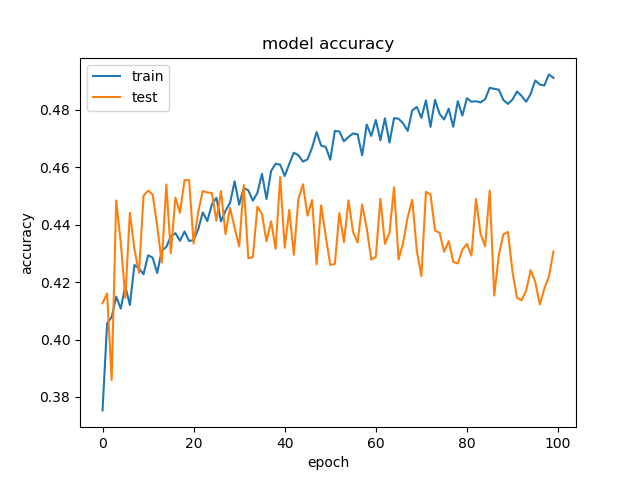
\includegraphics[width = 1.8in]{11.png}
    \caption{Model accuracy with pagerank}
\end{figure}
We choose the model with the least loss, the minimum loss is 0.139864, and the accuracy with this model is 0.402065.

\subsection{conclusion}
We can know from the the diagrams that with PageRank value added the accuracy can be improved greatly. Therefore, in the ranking of web pages, in addition to the relevance between query and web pages is very important, the relationship between nodes also has a great impact. It is possible that a node is not very relevant to the content we are searching for, but it links many highly relevant content, so its ranking will also be greatly increased.

\section{Summary}
We tried to combine the PageRank algorithm with Learning-To-Rank method in this project. And the result is relatively satisfactory, we can conclude from the diagrams that adding PageRank for ranking is beneficial.

In this project, we get familiar with Machine Learning algorithm and know more about Ranking for network,which will play an important role in our future learning. However, there are still pities during our project, such as at first, we are trying to implement PageRank algorithm in distributed file system, but due to time limit, we couldn't implement it. And the listnet didn't perform well in dealing with large amounts of data. The convergence speed of the ListNet algorithm is not fast. The running time depends directly on the size of the training set. It is not suitable for the training of data sets with large query volume. Maybe we will continue to optimize this project in our winter break.


Finally, we would thank Professor Jiang who gives us lots of advice about this project and gives us such a great chance to improve ourselves.



\begin{thebibliography}{99}  
\bibitem{ref1}Xinbo Ai,Node Importance Ranking of Complex Networks with Entropy Variation,Entropy 2017, 19, 303; doi:10.3390/e19070303

\bibitem{ref2}Yizhou Sun, Jiawei Han,Ranking Methods for Networks, ESNAM13.  

\bibitem{ref3}PageRank.  In Wikipedia, the free encyclopedia. Retrieved December 28,2018, from https://en.wikipedia.org/wiki/PageRank
 
 \bibitem{ref4}S. E. Robertson. Overview of the okapi projects. Journal
of Documentation. 1997; 53(1): 3~7.

\bibitem{ref5} Jay M. Ponte and W. Bruce Croft. A language modeling
approach to information retrieval. In Proceedings of
SIGIR 1998: 275~281

\bibitem{ref6} Evaluation measures (information retrieval).  In Wikipedia, the free encyclopedia. Retrieved October 2, 2018, from https://en.wikipedia.org/wiki/Evaluation\_measures\_(information\_retrieval)

\bibitem{ref7} Tao Qin, Tie-Yan Liu, Jun Xu, Hang LiLETOR: A benchmark collection for research on learning to rank for information retrieval, Springer Science+Business Media, LLC 2009

\end{thebibliography}

\end{document}

